\chapter{全景漫游与人的关系}

\section{全景漫游的生理行为特性}
实现全景漫游与传统人机界面最大的区别在于全景漫游时的设备(包括 VR 眼镜或专用眼罩)距离人眼只有 2~3 公分距离,设备整体对人眼呈包裹状态。使用者仅可通过听觉和其他一些不够灵敏的感觉来感受外界环境,使用环境的舒适性就变得非常重要。

全景漫游与人体关联的感觉和生理运动大致有:视觉、听觉、肢体运动等。如图\ref{fig:human_sence}。

\begin{figure}[htp]
\centering
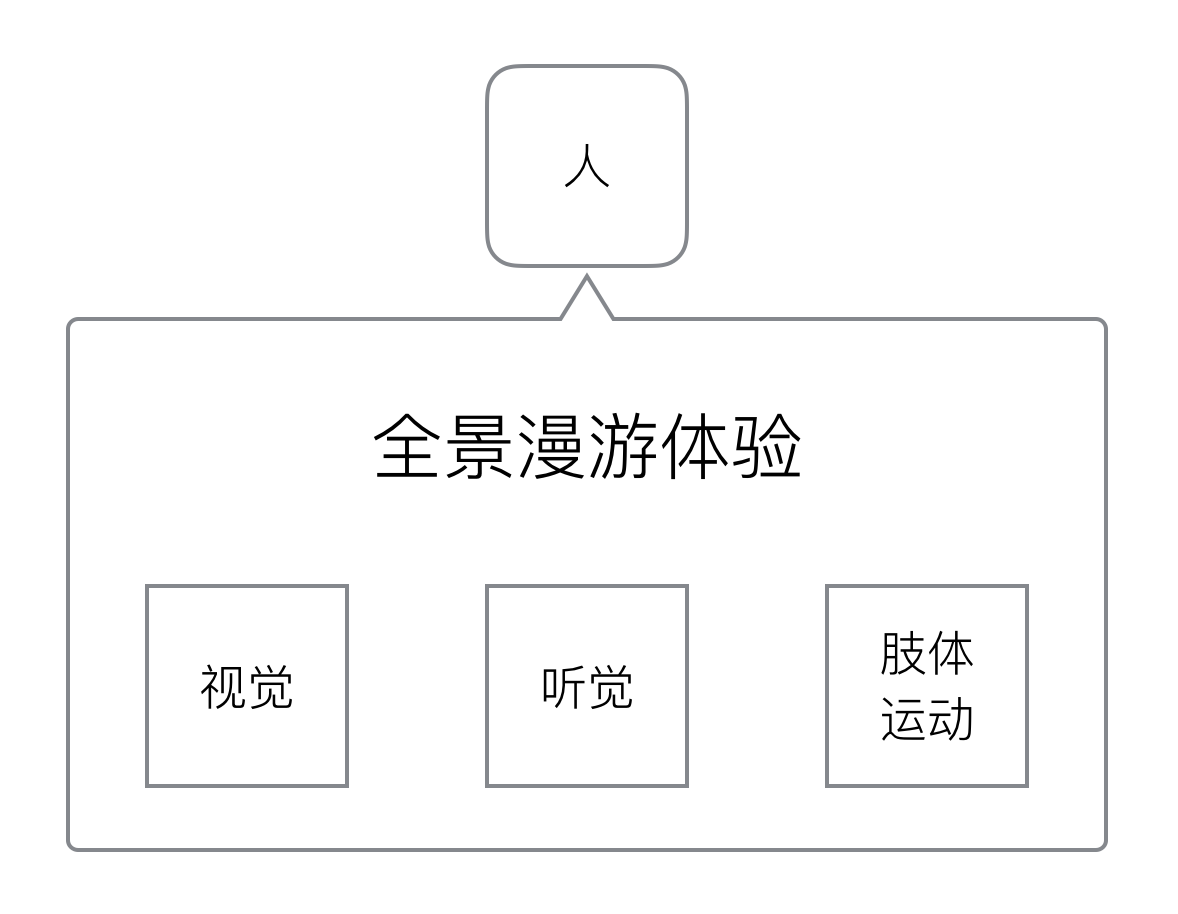
\includegraphics[width=.5\textwidth]{human_sence}
\caption{全景漫游与人体知觉}
\label{fig:human_sence}
\end{figure}

\subsection{全景漫游的视觉特征}
全景漫游对人体最大的刺激来源即是视觉刺激,其特征为距离眼睛距离近,色彩刺激较一般显示屏幕更为剧烈。

人的视角是确定被看物尺寸范围的两端点光线射入眼球的相交角度。视角的大小与观察距离及被看物体上两端点的直线距离有关,其计算公式\ref{eq:angle}如下:
\begin{equation}
\alpha=2\arctan{\frac{D}{2L}}
\label{eq:angle}
\end{equation}

如果设眼球距镜片距离为 1.5cm,而镜片上一物体显示高度为 2cm,则带入公式可得\ref{eq:data}

\begin{equation}
\alpha=2\arctan{\frac{2cm}{2*1.5cm}}\approx 67.38 ^{\circ}
\label{eq:data}
\end{equation}